\documentclass[a4paper]{article}
\usepackage[english]{babel}
\usepackage[utf8]{inputenc}
\usepackage{mdwlist}
\usepackage{paralist}
\usepackage{listings}
\usepackage[usenames,dvipsnames]{color}
\usepackage[bookmarks=true]{hyperref}
\hypersetup{
    unicode=false,          % non-Latin characters in Acrobat’s bookmarks
    pdftoolbar=true,        % show Acrobat’s toolbar?
    pdfmenubar=true,        % show Acrobat’s menu?
    pdffitwindow=false,     % window fit to page when opened
    pdfstartview={FitH},    % fits the width of the page to the window
    pdfkeywords={keywords}, % list of keywords
    pdfnewwindow=true,      % links in new window
    colorlinks=true,       % false: boxed links; true: colored links
    linkcolor=black,          % color of internal links
    citecolor=black,        % color of links to bibliography
    filecolor=black,      % color of file links
    urlcolor=black           % color of external links
}
\usepackage{tikz}
\usetikzlibrary{shapes,arrows,shadows,trees} % for pgf-umlsd
\usepackage[underline=true,rounded corners=false]{pgf-umlsd}

\lstset{ %
basicstyle=\footnotesize,       % the size of the fonts that are used for the code
numbers=left,                   % where to put the line-numbers
numberstyle=\footnotesize,      % the size of the fonts that are used for the line-numbers
stepnumber=5,                   % the step between two line-numbers. 
numbersep=5pt,                  % how far the line-numbers are from the code
backgroundcolor=\color{white},  % choose the background color. You must add \usepackage{color}
showspaces=false,               % show spaces adding particular underscores
showstringspaces=false,         % underline spaces within strings
showtabs=false,                 % show tabs within strings adding particular underscores
%frame=single,	                % adds a frame around the code
tabsize=2,	                % sets default tabsize to 2 spaces
captionpos=b,                   % sets the caption-position to bottom
breaklines=true,                % sets automatic line breaking
breakatwhitespace=false,        % sets if automatic breaks should only happen at whitespace
title=\lstname,                 % show the filename of files included with \lstinputlisting; also try caption instead of title
%escapeinside={\%*}{*)},          % if you want to add a comment within your code
inputencoding=utf8,
extendedchars=true
}

%highlight
%\usepackage{color}
%\usepackage{alltt}
%\usepackage{ucs}
%\input {highlight.sty}


\begin{document}
\title{Medical Expertise Ordering System}
\author{Seweryn Niemiec, Krzysztof Bogusławski,\\ 
Łukasz Martyniak, Bartosz Uchacz, Przemysław Wyrobek \\ 
\textbf{Academic Center of Computer Science } of \\ 
Westpomeranian University of Technology in Szczecin,\\
Fundacja IT}
\date{\today}
\maketitle
\tableofcontents
\listoffigures
\listoftables

\section{Versions of The Document}

This document describes version $1.0$ of the System.

\subsection{Third Edition}
\begin{description}
  \item[Date of creation] 2010-01-01
  \item[Status] working draft
  \item[Changes] \hfill \\
	\begin{enumerate}
      \item The System version numbers has been defined.
      \item The System and Document versions has been renumbered.
      \item The rules of maintenance of compatibility between the versions has been defined.
	  \item It has been specified that XML files do not use UTF BOM mark.
      \item New rule: clients and servers not supporting signatures shall 
		ignore the files containing signatures.
      \item New rule: in case of a faulty or incomplete signature an order is 
		automatically withdrawn through creation of an appropriate $comment$.
      \item A server SHOULD feature a capability of adding next CNs to the 
		list of authorized to access to a given order
      \item Support for DICOM attachements is now required, other formats allowed.
	\end{enumerate}
  \item[List of issues] \hfill \\
	\begin{enumerate}
      \item The name and surname are stored in a single XML element.
      \item Inconsistent elements featuring a person in XML documents.
	  \item Response to HTTP GET on directory resource is not specified.
	\end{enumerate}
\end{description}

\subsection{Second Edition}
\begin{description}
  \item[Date of creation] 2010-06-02
  \item[Status] working draft
  \item[Changes] \hfill \\
	\begin{enumerate}
      \item Declaration of the list of services has been added.
	  \item Support for \emph{xmldsig-core}, \emph{W3C XAdES 20030220} 
		and \emph{ETSI TS 101 903 V1.3.2} signing formats has been added.
	  \item Confirmation of acceptance of the order by the consultant has been specified.
	  \item Time-stamping has been defined.
      \item Support for \emph{pkcs\#7} has been removed.
      \item Support fot HTTPS as the method of transport is now required.
      \item Interpretation of an examination in now stored in DICOM SR.
      \item A date of realization of an examination has been added to the content of the order.
      \item Format of the resource references has been changed to URI.
      \item New rule: possibility of modification of the order which is in state \emph{created}
		is forbidden.
      \item 3 types of comments has been specified.
      \item An \emph{unspecified gender} has been added to the content of the 
			order in the \emph{Gender} field
      \item The \emph{id} attribute has been added to \emph{Patient} element in the content
			of the order. 
      \item \emph{Referral} element has been added to the content of the order.
      \item Subdirectories grouping orders by years has been added to the directory 
		structure.
	\end{enumerate}
\end{description}

\subsection{First Edition}
\begin{description}
  \item[Date of creation] 2010-05-14
  \item[Status] working draft
  \item[Changes] initial version
\end{description}

\section{Introduction}

Solution presented in this document is not a protocol, but rather a system. Medical
Expertise Ordering System (MEDEOS), called later the System, is a software solution for
medical documents interchange, with the primary focus on remote diagnosis and
teleradiology. The name of the System refers mainly to the primary goal of operation, 
i.e. electronic ordering of interpretations of radiologic examinations, but due to 
its flexibility the System can perform other functions in the future as well.

The key principles of the System are: 
\begin{inparaenum}[\itshape a\upshape)]
\item simplicity -- simple systems can be implemented at a low cost and are easy to
maintain,
\item flexibility -- to allow realization of new functions based on the same mechanism and
\item security -- required when transmitting sensitive personal data.
\end{inparaenum}

Currently, the functionality is as follows:
\begin{itemize}
  \item A medical unit can electronically order another unit to execute an interpretation of
  an medical examination;
  \item The order can have digital files attached to it (usually DICOM images, but any
  file is allowed);
  \item An entity making the interpretation, if necessary, can make comments to the ordering
  unit, indicating what corrections are expected;
  \item The ordering unit can correct the order and attachments;
  \item When interpretation is ready, the ordering unit can download it;
  \item The interpretation can have additional digital files attached to it;
  \item Data and communication are protected from access by unauthorized persons;
  \item The System supports digital signatures, but not enforces it.
\end{itemize}

This document is to be the basis for the implementation of the system, so the words MUST,
SHOULD, MAY etc. have to be understand as described in RFC2119 [6].

\subsection{Elements Of The System}

There are two kinds of actors: the \textbf{customer} who makes an \emph{order}
and the \textbf{consultant} carrying out the \emph{interpretation} of the examination.
There can be many \emph{customers} and many \emph{consultants} in one \emph{co-operation
network}.

\textbf{Co-operation network} is the collection of all nodes on which the System is
running and which are prepared (configured) to communicate with each other. It consists
of at least one \emph{client} type node and one \emph{server} type node. One node can
have client and server functionality.

Other definitions:
\begin{description}
  \item[order] the commission of interpretation of medical examination created by the
  \emph{customer}, send to \emph{consultant}
  \item[interpretation] interpretation of medical examinations performed by the
  \emph{consultant} in response to the received \emph{order}
  \item[attachment] a file of any content accompanying the \emph{order} or
  the \emph{interpretation}; usually in practice it will be a DICOM image created as a result
  of examination, that have to be described by the \emph{consultant} (attachments to the
  order) or where the \emph{consultant} has made notes (attachments to the
  \emph{interpretation})
  \item[comment] comments made by the \emph{consultant} to the \emph{customer}, indicating
  problems with the commission and what corrections in the \emph{order} are expected
  \item[client] software sending files to the \emph{server} and downloading
  results
  \item[server] software collecting \emph{orders} and providing them to the
  \emph{consultant interface} and collecting \emph{interpretations} and providing them
  to a \emph{client}
  \item[customer interface] software providing [graphical] user interface for 
  \emph{customer} and directing the \emph{client}
  \item[consultant interface] software which provides [graphical] user interface for
  \emph{consultant}, allows the \emph{consultant} to browse \emph{orders} on the
  \emph{server} and save \emph{interpretations} to it
\end{description}

\emph{Customer interface} and \emph{consultant interface} are not integral part of
the System, but are necessary for usability and users' comfort. Those are the only
\footnote{there is one exception} components which interpret the contents of transferred
files. The System is open to many ways of implementing and connecting booth components
with the \emph{client} and the \emph{server}. Appearance, method of presentation,
integration with other IT systems and functionality of those components will be determined by
individual users' needs.

\subsection{Guidelines}

The primary function of the System is to send orders to describe results of 
examinations from one medical unit to another. This is done as described below.

\begin{figure}[t]
  \centering
  \begin{sequencediagram}
    \newinst{zlec}{Bob:Customer}
    \newthread[green]{kli}{stationA:Client}
    \newthread[red]{ser}{stationB:Server}
    \newinst[1]{kons}{Alice:Consultant}
    
      \mess{zlec}{Enter order data}{kli}
      \begin{sdloop}{Completing order loop}
	      \mess{zlec}{Send order}{kli}
	      \begin{sdloop}{Sending order loop}
	        \begin{call}{kli}{PUT file}{ser}{}
	        \end{call}
		  \end{sdloop}
	      \mess{ser}{Notification}{kons}
	      \mess{kons}{Comments}{ser}
	      \begin{call}{kli}{GET status}{ser}{}
	      \end{call}
	      \mess{kli}{Notification}{zlec}
	      \mess{zlec}{Corrections}{kli}
	   \end{sdloop}
       \mess{kons}{Interpretation}{ser}
       \begin{sdloop}{Interpretation getting loop}
         \begin{call}{kli}{GET file}{ser}{}
	     \end{call}
	   \end{sdloop}
       \mess{kli}{Notification}{zlec}
  \end{sequencediagram}
  \caption{\label{fig:sesja}Typical session customer -- consultant.}
\end{figure}


\begin{enumerate}
  \item The \emph{customer}, using the \emph{customer interface}, enters information
  related to the \emph{order} and selects which files should to be attached to it.
  Among the information about the order there is the name of the medical unit
  (the \emph{consultant}) to which the order will be send.

  \item \label{enum:send} When all data has been completed, the \emph{customer} starts the
  procedure of \emph{order} sending. If an electronic signature is used, the
  \emph{customer} will be asked to sign the \emph{order} with their private key. Sending
  itself SHOULD be done in the background, to prevent blocking user interface. 
  
  \item Based on the name of the \emph{consultant}, the \emph{client} selects 
  appropriate \emph{server}’s address and sends all data there. Data can be transmitted in
  many parts. One part is one file.

  \item After receiving complete \emph{order}, the \emph{server} sends a notice to the
  \emph{consultant}.

  \item \emph{Consultant} analyzes the \emph{order} and creates a reply using 
  \emph{consultant interface}. There are two kinds of reply:
  \begin{description}
    \item[interpretation] -- the \emph{interpretation} of the examination result is created
    when the order has been completed successfully; the \emph{client} can
    download it at any time,
    \item[comment for customer] -- the \emph{comment} is created when, for some reason, the
    \emph{consultant} cannot create a \emph{interpretation};
    \emph{comment} can inform the \emph{customer} about necessary
    corrections in the \emph{order}; the \emph{client} can download the \emph{comment} 
    at any time,
  \end{description}

  \item The \emph{client} checks the \emph{server} periodically for a \emph{interpretation}
  or a \emph{comment}. One check per \emph{order}. If one of those files can be downloaded,
  then \emph{client} downloads it and creates a notice for the \emph{customer}.
 
  \item Downloading \emph{interpretation} finishes the \emph{order}. A \emph{comment} means
  that \emph{customer} should make corrections to the \emph{order} and go back to
  \mbox{point \ref{enum:send}}.
\end{enumerate}

Figure \ref{fig:sesja} shows a course of \emph{order} execution in graphical form.
There are two simple commands on a \emph{client} -- \emph{server} communication level:
send file (PUT) and get file (GET). File contents are transparent for commands and are not
interpreted by the System. The \emph{order} status is determined by the presence or
not of files on a \emph{server}. It's \emph{customer and consultant interfaces'} job
to understand and maintain the order's state. Commands can be realized by any transport
method, such as: HTTP, WebDAV, FTP, or even PenDrive or CD connected with manual file
moving. HTTPS is recommended as it allows easy implementation of security rules and simple
integration of custom and third party code (http servers as file servers). The main goal
of this document is to define the directory structure of an \emph{order}.

The System has to be secure, so that unauthorized persons have no access to the
transfered and stored data and users could not fake it's identity. 

\section{Versions of the System and Compatibility}
The version of the System consists of two numbers separated by dot, e.g. 1.0. The first, 
high-order digit is changed if any change violating compatibility with a previous version 
is implemented in the System. A change can be such modification of structure of an XML document
that the sense of a previously used element is changed or a new obligatory element is added. 
The second, low-order digit is changed if any change that does not violate backward 
compatibility is implemented. Such change can be adding an optional element to an XML file. 
The parties of the data exchange (client and server) implementing versions of the System with 
the same high-order digit SHOULD communicate without any problems.

The version of the system is recognized through testing of an XML namespace to which the root 
element of a processed XML document belongs. A namespace is created through adding a string 
denoting version and preceded by a letter of „v”, e.g. v1.0. A namespace for the System of 
the version 1.0 is: http://www.medeos.org/v1.0.

If any incompatibility is detected, at least one party of the data exchange MUST be informed. 
If any lack of compatibility is detected by the server, the server shall return to the client 
an appropriate HTTP error code and description.


\section{Features}

\subsection{Freedom of implementation}

The features of the System arise directly from the hereinafter described mechanism of operation.
The mechanism can be implemented in many ways. The simplest and fully functional implementation 
can be composed using the following components:
\begin{itemize}
  \item standard web server, like Apache lub IIS -- server has to have an option to
  attach your own implementation of HTTP PUT and DELETE methods (most popular web servers
  has this option),
  \item two CGI programs, written in any language, which handle PUT i DELETE methods on
  web server -- programs can be so simple that it is possible to create them as Unix
  shell scripts (examples of such scripts in languages such as Perl, PHP, VBScript are
  available on the Internet for Apache HTTP Server and MS IIS),
  \item filesystem with access control (operating systems such as Unix (and its
  derivatives) and MS Windows Server has it built-in),
  \item \emph{cURL} tool as a client -- this tool is freely available on GPL licence for
  most operating systems.
\end{itemize}

The System can also be implemented using more sophisticated solutions, like Java Servlets
and relative databases, but it has been designed to make it an option, not a requirement. 
The summary of the features of the System is presented below.

\subsection{Transparency}

The System is transparent for transportation methods and file contents. It means that the 
System operation does not depend on the method of transport of files and the content or 
format of transported filesfiles. File formats and transport methods can be changed in 
the future without any influence to mechanism operation.

\subsection{Stateless server}

The server is stateless, but the order has a state. The state of the Order is derived 
from the presence or not of specific files in order's directory
on the server. Client checks the state using GET command. An order can
have states such as: \emph{during creation}, \emph{ordered}, \emph{commented},
\emph{finished} \textbf{FIXME}. Due to the fact that transition of the state is caused by 
the appearance or disappearance of files, adding and removing files has to be an atomic 
operation. 

The communication itself between the nodes is stateless, and can be performed through stages, 
whereas a stage can be of any duration. There is no definition of the communication session
or transaction, therefore transport can be realized by means of physical relocation of mass
memories (e.g. CD).

\subsection{Scalability}

The System is highly scalable due to elimination of sharing and synchronization between the 
nodes belonging to the same cooperation network. The co-operation network has no central point. 
The only required global identifiers are clients' and servers' names (ip addresses, domain names 
or the Distinguished Name from Subject attribure of SSL Digital Certificate),
which are already unique. Every client cares for its own resources and manages them independently. 
Client can be identified on the server by its domain name or, in case of using HTTPS, by 
Subject attribute from client's digital certificate. There is no need for maintenance of any 
global ids.
	Lack of requirement of the central point does not mean that the cooperation network cannot
have its own center. The system makes it possible to create a central unit having functionality
of the client and server and performing functions such as:
\begin{itemize}
	\item mediation or coordination of exchange of data between other units,
	\item fulfillment of functions of the authorization center (CA) for the public key infrastructure (PKI) issuing digital certificates (X.509).
	\item fulfillment of time-stamping functions.
\end{itemize}

\subsection{Security}

Security is provided by user authentication, user authorization, transfer encryption and
file signing.

Method of \textbf{authentication} depends on a used file transfer mechanism and is provided
by this mechanism. In case of HTTPS and WebDav over HTTPS it will be mutual
authentication based on client's and server's certificates, in case of HTTP and FTP it will be
login and password authentication and in case of file moving using CD/Pendrive it can be
verification performed by sysadmin.

\textbf{Authorization} can be performed on the file access level, so it is independent of 
transportation method. Every client, which can communicate with the particular server, has 
its own directory on it. This directory groups all resources belonging to the client. Only 
this client and the consultant program have access to the directory. If the filesystem is used
as a database, authorization can be successfully performed by the mechanisms of access control
embedded into the server’s filesystem. In other cases the mechanisms embedded into the HTTP
server or own solutions in programs carrying out HTTP GET, PUT and DELETE methods can be used. 
and can be performed by:
custom code, web server (some web servers have sufficiently powerful configuration options to perform
this task) or filesystem's access control (when using filesystem as storage). Using
filesystem's access control mechanism is the easiest solution. Every client,
which can communicate with the particular server, has its own directory on it.
Clients can not access files in directories they do not own. Consultant interface has
special privileges and can access all files.

\textbf{Privacy} of transmission depends on the transport method. As for the methods not
guaranteeing confidentiality, it shall be provided at a lower layer (encrypted VPN networks).

\section{Mechanism of Operation}

\subsection{Client -- Server Communication}

Mechanism of communication has been developed considering HTTPS as a transportation method.
Using this method is probably the easiest way to implement rules described here.
Because the System works by moving or coping files, it is possible to use any other way to 
dislocate files to make the System work. For simplicity, this document takes HTTPS as a base
transportation method and filesystem as a storage. Except for special cases, the client-server 
communication SHOULD be performed by means of HTTPS. 

The Client and the sever communicate using three standard HTTP methods: GET, PUT and
DELETE. Implementation of those methods MUST comply to RFC2616. Client uses GET method to
get order state, comment and interpretation, PUT to send the order body and attachments and
DELETE to remove the comments. The program implementing mechanisms of the System provides 
realization of the functions PUT and DELETE on the server side. Handling the GET method 
returning files from the filesystem is embedded into every HTTP server, however, own 
implementation is often useful. Using HTTPS for security is described in section 
\ref{sec:bezp}.

URL address consists of the following components:
\begin{description}
	\item[protocol]	transport protocol; it SHOULD be HTTPS
	\item[server address]	domain name of the server
	\item[system name]	name of the System: „medeos”
	\item[service name]	in the future the System can realize various functions, ordering of 
		examinations defined in the document is identified by the word „order”
	\item[client name]	name of the client who created an order; the name MUST be used for 
		authorization of the clients; SHOULD be compared with Common Name from the certificate 
		used by the client for communication by means of HTTPS
	\item[year]	year of creation of an order; this component guarantees that the list of orders can be shortened if the server operates for many years
	\item[order ID]	identifier of an order; order ID is selected by the client
	\item[resource]	path indicating a specific resource as the element of an order; structure of resources is described in section 5.2
\end{description}

Example of URL:\\
\emph{https://example.com/medeos/order/szpital-X/2010/32434/body.xml}\\


The list of basic HTTP requests is presented below. If a digital signature is used, there
are extra requests related to transfer of files with signatures. Components of URL written
using italics and enclosed between $<$ and $>$ chars are variable elements and are replaced by 
a string identifying a specific resource name/id.

\begin{description}
  \item[GET /medeos/order/$<$\emph{client}$>$/]  \hfill \\
  Get a list of years during which the orders were submitted.

  \item[GET /medeos/order/$<$\emph{client}$>$/$<$\emph{year}$>$/]  \hfill \\
  Get a list of all orders submitted to the server by a given client in a given year.
  
  \item[PUT /medeos/order/$<$\emph{client}$>$/$<$\emph{year}$>$/$<$\emph{order id}$>$/$<$\emph{attachment}$>$] \hfill \\ 
  Send attachment to the server. Parent directories (\emph{order id} and \emph{year})
  are created on demand. If the given attachment does not exists it will be
  created else it will be overwritten. Overwritten files SHOULD be moved to
  the order history.
  
  \item[PUT /medeos/order/$<$\emph{client}$>$/$<$\emph{year}$>$/$<$\emph{order id}$>$/body.xml] \hfill \\ 
  Send order body to the server. Order body MUST be sent as the last file (after 
  attachments and signatures are delivered). The appearance of \emph{body} file is a 
  signal that complete order has been uploaded
  and server can send a notification to the consultant interface. 

  \item[GET /medeos/order/$<$\emph{client}$>$/$<$\emph{year}$>$/$<$\emph{order id}$>$/]  \hfill \\
  Get the list of order files. It can be used to check if complete order has been
  uploaded.

  \item[GET /medeos/order/$<$\emph{client}$>$/$<$\emph{year}$>$/$<$\emph{order id}$>$/response/]  
  Get the list of files created by a consultant as a response to an order. If there is a 
  file named ,,response.dicom'', the interpretation has been completed and the results can be 
  downloaded. If there is a file named ,,comments.xml", the consultant was unable to create 
  interpretation and provided notices for the customer. If interpretation contains 
  attachments, their names will be on the list.

  \item[GET /medeos/order/$<$\emph{client}$>$/$<$\emph{year}$>$/$<$\emph{order id}$>$/response/response.dicom] 
  Get an interpretation.
  
  \item[GET /medeos/order/$<$\emph{client}$>$/$<$\emph{year}$>$/$<$\emph{order id}$>$/response/comments.xml] \hfill \\
  Get a comment.

  \item[GET /medeos/order/$<$\emph{client}$>$/$<$\emph{year}$>$/$<$\emph{order id}$>$/response/$<$\emph{attachment}$>$] \hfill \\ 
  Get an interpretation attachment.

  \item[DELETE /medeos/order/$<$\emph{client}$>$/$<$\emph{year}$>$/$<$\emph{order id}$>$/response/comments.xml]\hfill \\ 
  Delete a comment. Deletion of the comments file is a signal that customer has applied to
  consultants comments (has made corrections to the order) and the order can be send
  for consultation again.

\end{description}

All changes made by PUT and DELETE methods SHOULD be logged in
\emph{/medeos/order/$<$\emph{client}$>$/$<$\emph{order id}$>$/history/log} file, which is
described in section \ref{sec:model}.

\subsection{Data Model}
\label{sec:model}
\begin{figure}
\centering
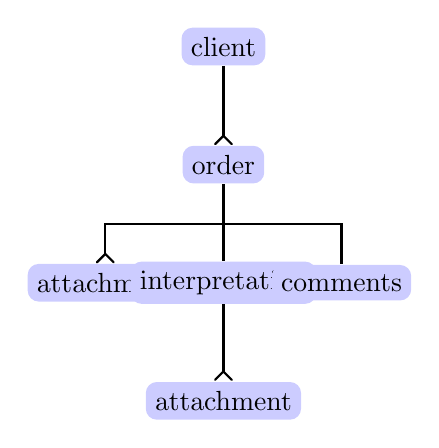
\begin{tikzpicture}
	[
	every node/.style={fill=blue!20,rounded corners},
	edge from parent/.style={-angle 90 reversed, thick, draw}	
	]
	\node {client}
		child {node {order}[style=edge from parent fork down]
			child {node {attachment} }
			child {node {interpretation} edge from parent [-butt cap]
				child {node {attachment} }
			}
			child {node {comments} edge from parent [-butt cap]}
		};
\end{tikzpicture}
\caption{\label{fig:modeldanych}Data model on a server.}
\end{figure}

System operates on four entities: order body, attachment, interpretation and comments which
are structured as a tree. Figure \ref{fig:modeldanych} shows its relations.
The tree structure with files as nodes can be successfully implemented using
filesystem as a database and this solution is referenced in following text. 

A directory structure implementing the data model of the server is presented below. Locations
and names of files are reflected in the URL addresses used by the client connecting by HTTP
to a server. Locations and names of files are reflected in URL addresses, which client
uses connecting by HTTP to a server. If a server does not use identical directory structure
as presented below, it MUST map its structure to URL paths, so that the client cannot see 
the difference.

\begin{description}
	\item[/medeos/order/$<$\textit{client}$>$/]
	Directory to which only the given client has access. The name of the directory identifies
	the client.

	\item[/medeos/order/$<$\textit{client}$>$/$<$\emph{year}$>$/]
	Directory grouping client's orders. It is created on demand when the client makes PUT to 
	a non-existing order directory in non-existing group.

	\item[/medeos/order/$<$\textit{client}$>$/$<$\emph{year}$>$/$<$\textit{order id}$>$]
	Directory with the order. It is created on demand when the client makes PUT to 
	a non-existing order directory.
		\begin{description}
		\item[$<$\textit{attachment 1}$>$]   
		\item[$<$\textit{\ldots}$>$]   
		\item[$<$\textit{attachment N}$>$] Order attachments. When an order is created, 
			the client MUST at first upload attachments to the server.
		\item[body.$<$\textit{sig\_ext}$>$] Digital signature of the order made by the 
			customer. Details in section 6.4.
		\item[body.xml] File named ''body.xml'' contains text of the order. It is XML file 
			described in section \ref{sec:formaty}; The appearance of ''body'' file is a 
			signal for consultant interface that the order has been succesfully uploaded 
			and can be executed by the a consultant.
		\item[response/] A directory containing response of the consultant. It is created on
			demand, when consultant saves a response.
			\begin{description}
			\item[confirm.$<$\textit{sig\_ext}$>$]
			Automatic electronic Signature made by the server, confirming the receipt of 
			order and binding the event with date and time. Details in section \ref{sec:sig}.
			\item[response.$<$\textit{sig\_ext}$>$]
			Digital signature of an interpretation made by the consultant. Details in section 
			\ref{sec:sig}.
			\item[response.xml] File ''response.xml'' contains the interpretation. It is XMl 
			file described
			in section \ref{sec:formaty}. The appearance of ''response.xml'' file is a signal for a
			client that a consultant has completed interpreting examination results. Client 
			can download this file at
			any time and present its contents to a customer via customer interface.
			The emergence of "response.dicom" file, transits order state to \emph{finished}.

			\item[comments.xml] File ''comments.xml'' contains consultant comments for the customer. 
			It can be created instead of ''response.xml'' file as a result of consultant work. 
			It is XML file described in section \ref{sec:formaty}. The appearance of this file 
			is a signal for the client that the consultant cannot perform an interpretation 
			for some reason. Client MUST download this 
			file and show its contents to the
			customer using customer interface. Comments should help customer to make right
			corrections to the order. When the order will be revised according to the 
			consultant's comments, the file ''comments.xml'' MUST be deleted by the customer.
			It will be a signal, that order can be send to consultation again;
			\item[$<$\textit{attachment 1}$>$]   
			\item[$<$\textit{\ldots}$>$]   
			\item[$<$\textit{attachment N}$>$] Files attached to an interpretation. 
			Interpretation attachments MUST be created before ''response.xml'' file,
			\end{description}
		\item[history/] Order's history. This directory contains files deleted or
		overwritten by the client. When client destroys any file, it is moved to this
		directory. New name of the moved file is constructed by adding a date and time to
		the original file name. Time SHOULD be represented in ISO format 
		(YYYY-MM-DDThh:mm:ss.sTZD)
			\begin{description}
  			\item[log] file named „log” contains history of the order; it is an XML file 
			which format has been described in section \ref{sec:formaty}. Every time any 
			change occurs in an order (a file is added, upated or deleted), a new entry with 
			information about an event appears in the „log”. This is the only file interpreted 
			by the server. 
			\end{description}
		\end{description}
\end{description}

Example of the directory structure with one order is presented in table \ref{tab:dir}.

\begin{table}
\begin{center}
\begin{tabular}{ p{2cm} p{.2cm} p{.2cm} p{.2cm} p{4cm} }
  \multicolumn{5}{l}{\textbf{/medeos/order}/spk1.szczecin.pl/1248/} \\
   & & & \multicolumn{2}{l}{\textcolor{gray}{156345-345.dicom}} \\
   & & & \multicolumn{2}{l}{\textcolor{gray}{453346.dicom}} \\
   & & & \multicolumn{2}{l}{\textbf{body}} \\
   & & & \multicolumn{2}{l}{\textcolor{gray}{dodatek.pdf}} \\
   & & & \multicolumn{2}{l}{\textcolor{gray}{rtg12.dicom}} \\
   & & & \multicolumn{2}{l}{\textbf{response}/} \\
   & & & & \textcolor{gray}{156345-345-v2.dicom} \\
   & & & & \textbf{response.xml} \\
   & & & \multicolumn{2}{l}{\textbf{history}/} \\
   & & & & \textbf{log} \\
\end{tabular}
\caption[Example finished order]{Example of the finished (with interpretation)
order. The interpretation has one attachment. Files which names are keywords are
shown in bold.}
\label{tab:dir}
\end{center}
\end{table}

\subsection{States Machine}

\begin{figure}
\centering
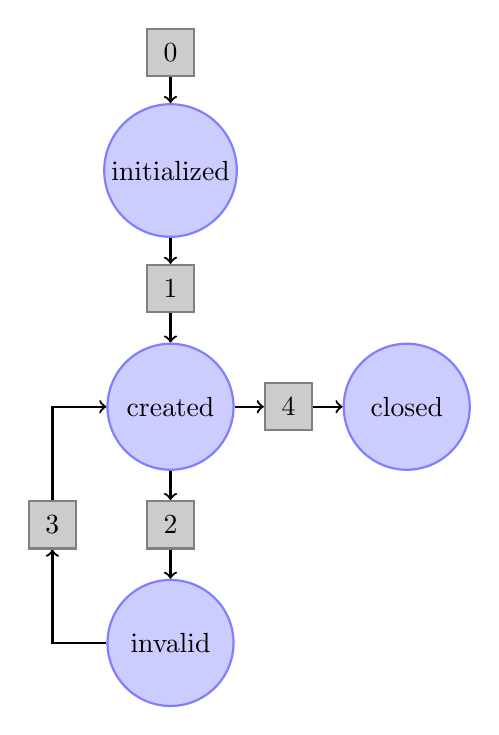
\begin{tikzpicture}
  [state/.style={circle, minimum size=16mm, 
  				node distance=1.5cm, inner sep=2pt, pin distance=4mm, 
  				draw=blue!50,fill=blue!20,thick
                },
   action/.style={rectangle, minimum size=6mm, 
  				node distance=1.5cm, inner sep=2pt, pin distance=4mm, 
  				draw=black!50,fill=black!20,thick
                }
                  ]
  \node[action] (a0) {0};
  \node[state] (init) [below of=a0]{initialized};
  \node[action] (a1) [below of=init]{1};
  \node[state] (cr) [below of=a1]{created};
  \node[action] (a2) [below of=cr]{2};
  \node[action] (a4) [right of=cr]{4};
  \node[state] (cl) [right of=a4]{closed};
  \node[state] (inv) [below of=a2]{invalid};
  \node[action] (a3) [left of=a2]{3};
  \draw[->, thick] (a0.south) -- (init.north);
  \draw[->, thick] (init.south) -- (a1.north);
  \draw[->, thick] (a1.south) -- (cr.north);
  \draw[->, thick] (cr.south) -- (a2.north);
  \draw[->, thick] (a2.south) -- (inv.north);
  \draw[->, thick] (inv.west) -| (a3.south);
  \draw[->, thick] (a3.north) |- (cr.west);
  \draw[->, thick] (cr.east) -- (a4.west);
  \draw[->, thick] (a4.east) -- (cl.west);
\end{tikzpicture}
\caption[Order's states]{Order's states. 0 -- creation of new order's directory; 1 --
creation of ''body.xml'' file; 2 -- creation of ''comments.xml'' file; 3 -- deletion of 
''comments.xml'' file; 4 -- creation of ''response.xml'' file.}
\label{fig:stany_zlec}
\end{figure}

A server, which is in fact a file server with predefined directory structure, does not 
analyze its own or order's state as it is a task for the customer and the consultant interface.
Possible order states are shown in figure 3. Transitions between states are triggered by 
an appearance (or disappearance) of files. Depending on the method of change detection, 
it may be necessary to provide atomicity to files adding to the order directory. The state 
change MUST occur only after the complete file is put into the structure.

\subsection{Services Dictionary}

The consultant MUST provide the list of services offered. The list of services is 
maintained on the server in the file \textit{/medeos/order/\textbf{services.xml}}. It is an 
XML file described in section \ref{sec:formaty}. Service name is part of the order's text.
During creation of an order body, the customer puts the name of the selected service into 
the body. If an order with the service name out of the list is detected on the server, the 
consultant (or the server automatically) should indicate in the comment that the order has 
to be corrected. In practice, the services are in accordance with the described types of 
examinations.

\section{Security}
\label{sec:bezp}

Security is realized on four tiers: client authentication on a server, access authorization, 
confidentiality of transmission and digital signatures of orders and interpretations. 
HTTPS and X.509 certificates SHOULD be used for authentication and confidentiality. It is a 
solution of a high level of security and easy for implementation.

TODO: description of files signing.

\subsection{Client Authentication} 

The goal of client authentication is the protection of data from unauthorized access and
unequivocal link on the recived data with the institution that sent them.
Authentication method depends on a file transportation
protocol. It can be based on digital certificates or logins and passwords, but to easy
integration clients nad servers SHOULD use certificates and HTTPS.

\subsection{Authorization}

The goal of authorization is protection of data from unauthorized access and protection
of server's directory structure from corruption. If HTTP[S] is used for transport of files, 
authorization of the client can be performed by a web server or by CGI programs handling GET, 
PUT and DELETE requests. The basic verification is carried out through comparison of CN from 
the client certificate with the client name included in URL of an order. The server SHOULD 
be also able to add successive CNs to the list of authorized to access to a given directory 
with an order. Independently of the transport method, authorization can be performed through 
access control mechanisms built into the filesystem. In practice both methods will be combined. 
Access rules for individual resources are as follows:
\begin{description}
  \item[/medeos/order/$<$\textit{client}$>$/]\hfill\\
  A single designated client and consultant interface have access to the directory. The 
  client can read and write in this directory, whereas the consultant interface can only read.
  \item[/medeos/order/$<$\textit{client}$>$/$<$\textit{order id}$>$/response/]\hfill\\ 
  Client can read this directory and delete ''comments'' file. Consultant interface can
  read and write here.
  \item[/medeos/order/$<$\textit{client}$>$/$<$\textit{order id}$>$/history/]\hfill\\ 
  Client and consultant interface can only read here. 
\end{description}

\subsection{Transmission Confidentiality}

Confidentiality of transmission SHOULD be provided by appropriate encryption algorithms. 
It is recommended to use AES with a key of at least 128 bits. Thereby, it is recommended 
to use HTTPS with configuration of the server allowing connections only by means of AES 128 
bit or better. As for the use of protocols without encryption support, confidentiality 
should be ensured through use of encrypted tunnels or VPN.

\subsection{Digital Signatures}
\label{sec:sig}

It is possible that the customer and consultant decide to use a digital certificate in order 
to confirm authorship and data integrity. Digital signatures are not necessary for the operation 
of the System, and are only a protection for the communicating parties in matters of dispute. 
The parties that do not support signatures MUST ignore files containing signatures. In order 
to increase transparency, the signatures are realized in \emph{detached} form, i.e. are stored 
in separate files regardless of the data files. The name of the file with signature is created 
by adding an appropriate extension to the name of the signed file. The extension depends on 
the format used to store the signature.

The following types of signatures are permitted:
\begin{description}
\item W3C xmldsig-core 20080610 – file extension .xmldsig.xml
\item W3C XAdES 20030220 – file extension .xades.xml
\item ETSI TS 101 903 V1.3.2 – file extension .etsi-ts-101-903.xml      
\end{description}

It is recommended to use XAdES or ETSI TS 101 903 format.

The file with the signature shall contain URIs and checksums of the signed files and 
X509v3 certificate of the signatory (containing a public key corresponding to the private key 
used for signing) for verification of the signature.

Only the following files are signed: body.xml – order body, response.xml – interpretation 
and comments.xml – comment of the consultant and its attachments. Attachments do not have 
separate sign files, but rather are signed together with the leading file to which they 
refer, through the use of extra Reference elements in leading file's signature.

A new signature shall be prepared after every change in the signed file and it shall be put 
into the server. It refers also to changes in attachments. The replaced files with signatures 
MUST be moved to the history directory.

If a directory with the signed order or a directory with the signed interpretation contains 
unsigned files, it is accepted that verification of the signature has failed.

\subsubsection{Binding of Files for xmldsig-core}

Binding of files (attachments to a leading file) is performed through creation of many 
Reference instances in the SignedInfo object. An URI attribute MUST contain an absolute and 
complete URL address pointing a file to which the hash defined in DigestValue refers.

\subsubsection{Binding of Files for ETSI TS 101 903}

Similarly as for \emph{xmldsig-core}.

\subsubsection{Binding of Files for XAdES}

Similarly as for \emph{xmldsig-core}.

\subsubsection{Time-stamping}

The system enables time-stamping of the created files in connection with the digital signature.
XAdES and ETSI TS 101 903 standards specify the methods of signature time-stamping and it 
is recommended to proceed according to the rules defined in these standards. Selection of
concrete signature format (XAdES-T, XAdES-C, XAdES-X, XAdES-BES, etc.) lies in hands of 
cooperation network members. Support for at least XAdES-T is recommended. 

If Time-Stamp Protocol (RFC 3161) is not used, a XAdES \emph{SigningTime} element 
shall be provided by a signatore himself. The signatory 
declares that the signature has been made no sooner than at the time specified in SignatureTime. 
Another party (verifying time stamp) is obliged to verify the time specified in SignatureTime. 
The verification SHOULD be performed automatically in accordance with the politics of an 
entity using the System. In case of claims related to the time entered, another party shall 
be immediately informed about the problem.

Time-stamping is not necessary for operation of the System and is only a protection for 
the parties communicating in matters of dispute.

\subsubsection{Confirmation of Acceptance of The Order}

If the client and server decide to use the digital signature, the server MUST create a 
digital signature confirming acceptance of the order. The confirmation is performed by 
signing a file with the signature made by the customer and storing it in the 
confirm.<sig ext> file described in section 5.2. The signature MUST be created automatically 
and immediately after the complete order has been received by the server. The signature 
confirming acceptance of the order MUST contain the signature date and time.

\subsection{Order History}

Modified or deleted files as the elements of the order are not lost irrevocably, but MUST 
be saved by the server to 
\textbf{.../$<$\textit{order id}$>$/history/}. The name of 
the saved file is created 
by adding modification date and time to the original file name. The time SHOULD be 
written in the format according to ISO 8601 format YYYY-MM-DDThh:mm:ss.sTZD.

\section{File Formats}
\label{sec:formaty}

The System interferes only with one file, i.e., \newline
,,/medeos/order/$<$\textit{client}$>$/$<$\textit{order id}$>$/history/log''. \newline
Contents of all other files
is interpreted and processed only by the user interfaces. In order to make the customer and 
consultant interfaces cooperate, the formats of files with order, interpretation and comment 
shall be fixed.

The general settlements about XML format are as follows:
\begin{itemize}
	\item All files of XML format MUST feature char coding in the UTF-8 standard;
	\item The file shall not contain UTF BOM mark;
	\item Strings of white marks following a mark closing an element and preceding a 
		mark opening an element SHOULD be ignored.
\end{itemize}

The interface of the customer and consultant MUST support attachments of DICOM format. 
Attachments in other formats can be sent as well. If the customer sends an attachment of the 
format not supported by the server, the server SHOULD automatically issue a comment with the 
information about lack of support of the file format.

\subsubsection{Structure of XML Documents}

Structure of XML files is defined in separate XML Scheme files.

\end{document}

